%------------------------------------------------------
%Author             : Daniel Schembri, Jonathan Schwarz
%University         : Pforzheim University
%Date of last edit  : Wed, 03 Sep 2014 14:12:16 +0200
%Filename           : multithreading_with_posix_pthreads.tex
%------------------------------------------------------

\documentclass[10pt,a4paper,DIV=11]{scrreprt}

%British English
\usepackage[UKenglish]{babel}
%utf8
\usepackage[utf8]{inputenc}

%pseudo-code
\usepackage[boxruled,vlined]{algorithm2e}

%for source code listings
\usepackage{listings}

\usepackage[table]{xcolor}

%tikz
\usepackage{tikz}
\usetikzlibrary{arrows,positioning,fit}

%plots
\usepackage{pgfplots}

%blocks - used by tikz-uml, included before
\pgfdeclarelayer{background}
\pgfdeclarelayer{foreground}
\pgfsetlayers{background,main,foreground}

%<,> in tikz-uml
\usepackage[T1]{fontenc}
\usepackage{tikz-uml}

%subfigure
\usepackage{graphicx}
\usepackage{subfigure}

%prevent figure from floating pictures
\usepackage{float}

%footer & header
\usepackage{fancyhdr}

%push footer down
\usepackage[bottom]{footmisc}

%footer & header
\pagestyle{fancy}
%clean footer & header
\fancyhf{}

%bibtex
\usepackage[square,numbers]{natbib}
\usepackage{gensymb}

%equation
\usepackage[tbtags]{amsmath}
\usepackage{amssymb} 

%table of contents with hyperlinks
%always include as last package
\usepackage{hyperref}

%===========================TITLE PAGE=======================================

%university logo
\titlehead
{
    
\includegraphics[width=0.20\textwidth]{files/hspflogo.pdf}\\

    Pforzheim University\\
    School of Engineering\\
}

\subject{Project work}
	
\title
{
    Evolving neutral networks\\
}

\author
{
    by \textbf{Daniel Schembri} - matriculation number: 310026 \\
    and \textbf{Jonathan Schwarz} - matriculation number: 304728
}
\date
{
    Winter term 2013/2014
}
%\today{}}

\publishers
{
    Examiner: Prof. Dr. rer. nat. Richard Alznauer\\
    Supervisor: Dr.Ing. Christoph Ussfeller
}


%=========================================GLOBAL SETTINGS=========================================

%footer &header

%\fancyfoot[L]{\textbf{Multi-Threading mit POSIX-pThreads}}
\fancyhead[R]{Page \thepage}
%\fancyhead[L]{\thechapter}

%chapter number and title
\fancyhead[L]{\nouppercase{\leftmark}}
%line
%\renewcommand{\footrulewidth}{0.5 pt}
\usepackage{lmodern}
\addtokomafont{sectioning}{\rmfamily}
\setlength{\parindent}{0mm}

%colour definitions
\definecolor{dkgreen}{rgb}{0,0.6,0}
\definecolor{gray}{rgb}{0.7,0.7,0.7}
%medium gray
\definecolor{mgray}{gray}{0.80}
%light gray
\definecolor{lgray}{gray}{0.97}

%hyperlink settings
%frame around hyperlinks
\hypersetup
{
    colorlinks = false,
    linkcolor = black,
    hypertexnames = false,
    citecolor = green
}

%listing settings
\lstset
{ 
    language=C,                
    basicstyle=\footnotesize\ttfamily,           
    numbers=left,
    stepnumber=5,    
    firstnumber=1,
    numberfirstline=true                 
    numberstyle=\color{black},                 
    numbersep=5pt,                 
    backgroundcolor=\color{white},      
    showspaces=false,             
    showstringspaces=false,         
    showtabs=false,                
    frame=single,                   
    rulecolor=\color{black},       
    tabsize=2,                     
    captionpos=b,                   
    breaklines=true,                
    breakatwhitespace=false,       
    title=\lstname,                    
    keywordstyle=\color{blue},          
    commentstyle=\color{dkgreen}, 
    identifierstyle=\color{black},      
    stringstyle=\color{purple},      
    escapeinside={\%*}{*)},      
    morekeywords={*,...},            
    deletekeywords={...}             
}

%=====================================DOCUMENT START=========================
\begin{document}

\tikzstyle{line}=[draw]
\tikzstyle{arrow}=[draw, -latex] 

%\renewcommand*\contentsname{Content}
%\renewcommand*\listtablename{Tables}
%\renewcommand*\listfigurename{Figures}
%\renewcommand*\bibname{Literature references}

\maketitle
\thispagestyle{empty}
\newpage
{\large\tableofcontents}
\newpage

\chapter{Artifical neural networks}
\section{Artifical neural networks}
The wish to build reproduce human intelligence has been around since the dawn of mankind. In the effort of building truely intelligent systems, thinking about our brain has turned out to be very useful, helping scientists to extent the scope of technical ideas to do so. One of the basic findings of neuron science is a hypohesis, which suggesst that mental acivity consists primarily of electrochemical acivity in large networks of brain cells, or neurons. Hence the name called neuronal networks. Let's take a look on the biological neuron in deatails. Figure \ref{fig:neuron} introduces the different parts of a neuron. Branching out from the Soma or cell body, several fibers called dendrites can be observed. The axon is a single long fiber with a length of 1 cm, is typically 100 times the diameter of the cell body. As a matter of fact, it can reach up to one meter. Up to 100,000 other neurons connect via the synpatic erminals at the end of the axon, building a neural network. Signals between neurons are transmitted between the network through a complicated chemical reaction. However, not every input has the same significance. In fact, the synapses amplify or reduce the signal strength of each connection, which enables the network control brain acivity in both the short term, and also long-term changes in the connectivity of neurons.

\begin{center}
\begin{figure}[H]
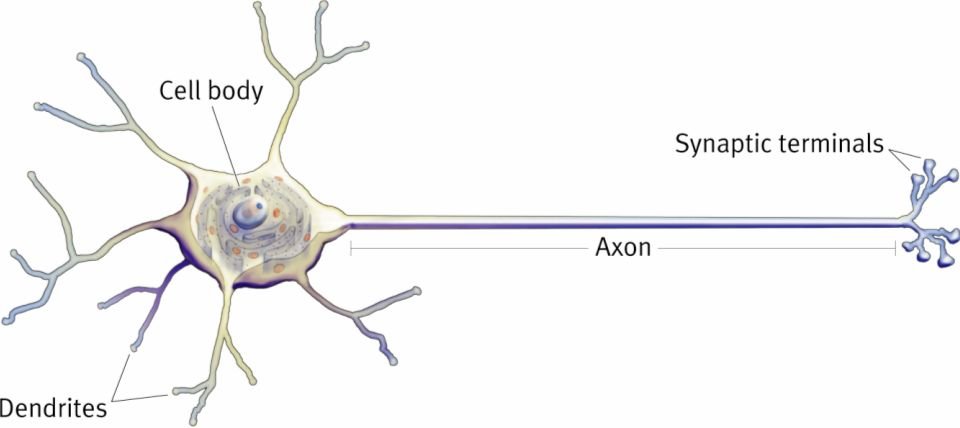
\includegraphics[width=0.8\textwidth,scale=1]{files/neuron.jpg}  
\caption{The parts of a nerve cell or neuron as shown in \cite{NEU}.}
\label{fig:neuron}
\end{figure}
\end{center}

Inspired by his hypothesis, some of the earliest work in the field of Artifical Intelligence aimed on building a similar srucure, a so called artifical neural network. The general idea of this approach perceives the neuron as a basic Input-Ouput unit, which somehow processes the signals of other neurons and propagades its result further into the network. The funcion of synpasis is simply reproduced by altering each individual input by a  factor which is constantly modified by a certain percentage. This never-ending modificaion of all the input weights represents the learning effect of an artifical neuron. A simple mathematical model of a neuron was first devised by \cite{NEURONMATH}.

\begin{figure}[H]
\centering

\begin{tikzpicture}
\node [align=center] (in1) at (-0.5,0) {$a_i$}; 
\node [align=center] (in2) at (-0.3,0.75)   {}; 
\node [align=center] (in3) at (-0.8,1.5) {$a_i = 1$}; 
\node [align=center] (w1) at (0.7,0) {$w_{ij}$}; 
\node [align=center] (w3) at (0.7,1.5) {$w_{0j}$};
\node [align=center] (input) at (2,0.75) {$\sum_{}^{in_{j}}$}; 
\node [align=center] (function) at (4,0.75) {$g()$}; 
\node [align=center] (output) at (6,0.75) {$a_j$}; 
\node [align=center] (o1) at (8.5,0) {};
\node [align=center] (o2) at (8.5,0.75) {};
\node [align=center] (o3) at (8.5,1.5) {};

\node [align=center] (desilinks) at (0,-1) {Input\\ Links}; 
\node [align=center] (desinput) at (1.9,-1) {Input\\ funcion}; 
\node [align=center] (desfunc) at (4,-1) {Activation\\ function}; 
\node [align=center] (desoutput) at (6,-1) {Output}; 
\node [align=center] (desolinks) at (8,-1) {Output\\ links}; 

\node [align=center] (desweight) at (4,2) {$a_j = g(in_j)$}; 
\node [align=center] (desinfunc) at (0.75,2) {\small Bias Weight}; 
\node [align=center] (descneuron) at (6,1.5) {\small \textcolor{red}{Cell body}}; 

\node [align=center] (dummy1) at (2.4,0.75) {}; 
\node [align=center] (dummy2) at (5.36,0.75) {}; 

\draw[arrow]	(in1) -- (input);
\draw[arrow]	(in2) -- (input);
\draw[arrow]	(in3) -- (input);

\draw[arrow]	(output) -- (o1);
\draw[arrow]	(output) -- (o2);
\draw[arrow]	(output) -- (o3);

\node[draw=red,fit=(dummy1) (function) (dummy2) ,ellipse] (tmp) {};

\end{tikzpicture}
\caption{A simple mathematical model for a neuron}
\label{fig:procthread}
\end{figure}


\subsection{Artifical neural networks}
%...
\section{Learning rules}
\subsection{Backpropargation}
%...
\section{Network tpyes}
\subsection{Feed Forward}
%...
\section{Applications}
\subsection{Pattern recognition}
%...

\KOMAoptions{listof=leveldown}

\newpage

%=========================================LISTS=========================================

\listoffigures
\listoftables
\listofalgorithms
\lstlistoflistings

\newpage

%=========================================DICTIONARY====================================

%dictiary style
\bibliographystyle{./files/alphadin}
%dictionary source
\bibliography{./files/bibdb}

\end{document}
